%%%%%%%%%%%%%%%%%%%%%%%%%%%%%%%%%%%%%%%%%
% Jacobs Landscape Poster
% LaTeX Template
% Version 1.1 (14/06/14)
%
% Created by:
% Computational Physics and Biophysics Group, Jacobs University
% https://teamwork.jacobs-university.de:8443/confluence/display/CoPandBiG/LaTeX+Poster
% 
% Further modified by:
% Nathaniel Johnston (nathaniel@njohnston.ca)
%
% This template has been downloaded from:
% http://www.LaTeXTemplates.com
%
% License:
% CC BY-NC-SA 3.0 (http://creativecommons.org/licenses/by-nc-sa/3.0/)
%
%%%%%%%%%%%%%%%%%%%%%%%%%%%%%%%%%%%%%%%%%

%----------------------------------------------------------------------------------------
%	PACKAGES AND OTHER DOCUMENT CONFIGURATIONS
%----------------------------------------------------------------------------------------

\documentclass[final]{beamer}

\usepackage[size=custom,width=142,height=107,scale=1.25]{beamerposter} % Use the beamerposter package for laying out the poster

\usepackage[none]{hyphenat} %Remove hypens

\usetheme{confposter} % Use the confposter theme supplied with this template

\setbeamercolor{title in headline}{fg=black,bg=black} % Colors of title headline and underline
\setbeamercolor{block title}{fg=black,bg=white} % Colors of the block titles
\setbeamercolor{block body}{fg=black,bg=white} % Colors of the body of blocks
\setbeamercolor{block alerted title}{fg=black,bg=nyellow!70} % Colors of the highlighted block titles
\setbeamercolor{block alerted body}{fg=black,bg=nyellow!10} % Colors of the body of highlighted blocks
% Many more colors are available for use in beamerthemeconfposter.sty

%-----------------------------------------------------------
% Define the column widths and overall poster size
% To set effective sepwid, onecolwid and twocolwid values, first choose how many columns you want and how much separation you want between columns
% In this template, the separation width chosen is 0.024 of the paper width and a 4-column layout
% onecolwid should therefore be (1-(# of columns+1)*sepwid)/# of columns e.g. (1-(4+1)*0.024)/4 = 0.22
% Set twocolwid to be (2*onecolwid)+sepwid = 0.464
% Set threecolwid to be (3*onecolwid)+2*sepwid = 0.708

\newlength{\sepwid}
\newlength{\onecolwid}
\newlength{\twocolwid}
\newlength{\threecolwid}
\setlength{\paperwidth}{56in} % A0 width: 46.8in
\setlength{\paperheight}{42in} % A0 height: 33.1in
\setlength{\sepwid}{0.024\paperwidth} % Separation width (white space) between columns
\setlength{\onecolwid}{0.22\paperwidth} % Width of one column
\setlength{\twocolwid}{0.464\paperwidth} % Width of two columns
\setlength{\threecolwid}{0.708\paperwidth} % Width of three columns
\setlength{\topmargin}{-0.5in} % Reduce the top margin size
%-----------------------------------------------------------

\usepackage{graphicx}  % Required for including images
\graphicspath{{images/}}

\usepackage{booktabs} % Top and bottom rules for tables

%----------------------------------------------------------------------------------------
%	TITLE SECTION 
%----------------------------------------------------------------------------------------

\title{Brew It Yourself} % Poster title

\author{Kevin Nause, Mathieu Tremblay, Scott Wood, and Steve Jung} % Author(s)

\institute{Department of Electrical and Computer Engineering, University of Waterloo} % Institution(s)

%----------------------------------------------------------------------------------------

\begin{document}

\addtobeamertemplate{block end}{}{\vspace*{2ex}} % White space under blocks
\addtobeamertemplate{block alerted end}{}{\vspace*{2ex}} % White space under highlighted (alert) blocks

\setlength{\belowcaptionskip}{2ex} % White space under figures
\setlength\belowdisplayshortskip{2ex} % White space under equations

\begin{frame}[t] % The whole poster is enclosed in one beamer frame

\begin{columns}[t] % The whole poster consists of three major columns, the second of which is split into two columns twice - the [t] option aligns each column's content to the top

\begin{column}{\sepwid}\end{column} % Empty spacer column

\begin{column}{\onecolwid} % The first column

%----------------------------------------------------------------------------------------
%	MOTIVATION
%----------------------------------------------------------------------------------------

\begin{block}{Motivation}

The traditional method for homebrewing requires various components, constant monitoring and heavy maintenance. There should be a solution which reduces complexity, making it much more affordable and practical for home use. The hope is to create a single vessel system that would make the home brewing process precise, automated and compact, all at a reasonable price.

\end{block}

%----------------------------------------------------------------------------------------
%	OBJECTIVE
%----------------------------------------------------------------------------------------

\begin{block}{Objective}

Combine homebrewing experience with engineering design, and construct a single vessel brewing system. By maintaining a strict control of key parameters, the brewing process is regulated using a combination of fluid mechanics, heat transfer, digital controls, power systems, embedded robotics and mobile development.

\end{block}

%----------------------------------------------------------------------------------------
%	BLOCK DIAGRAM
%----------------------------------------------------------------------------------------

\begin{block}{Block Diagram}

\begin{figure}
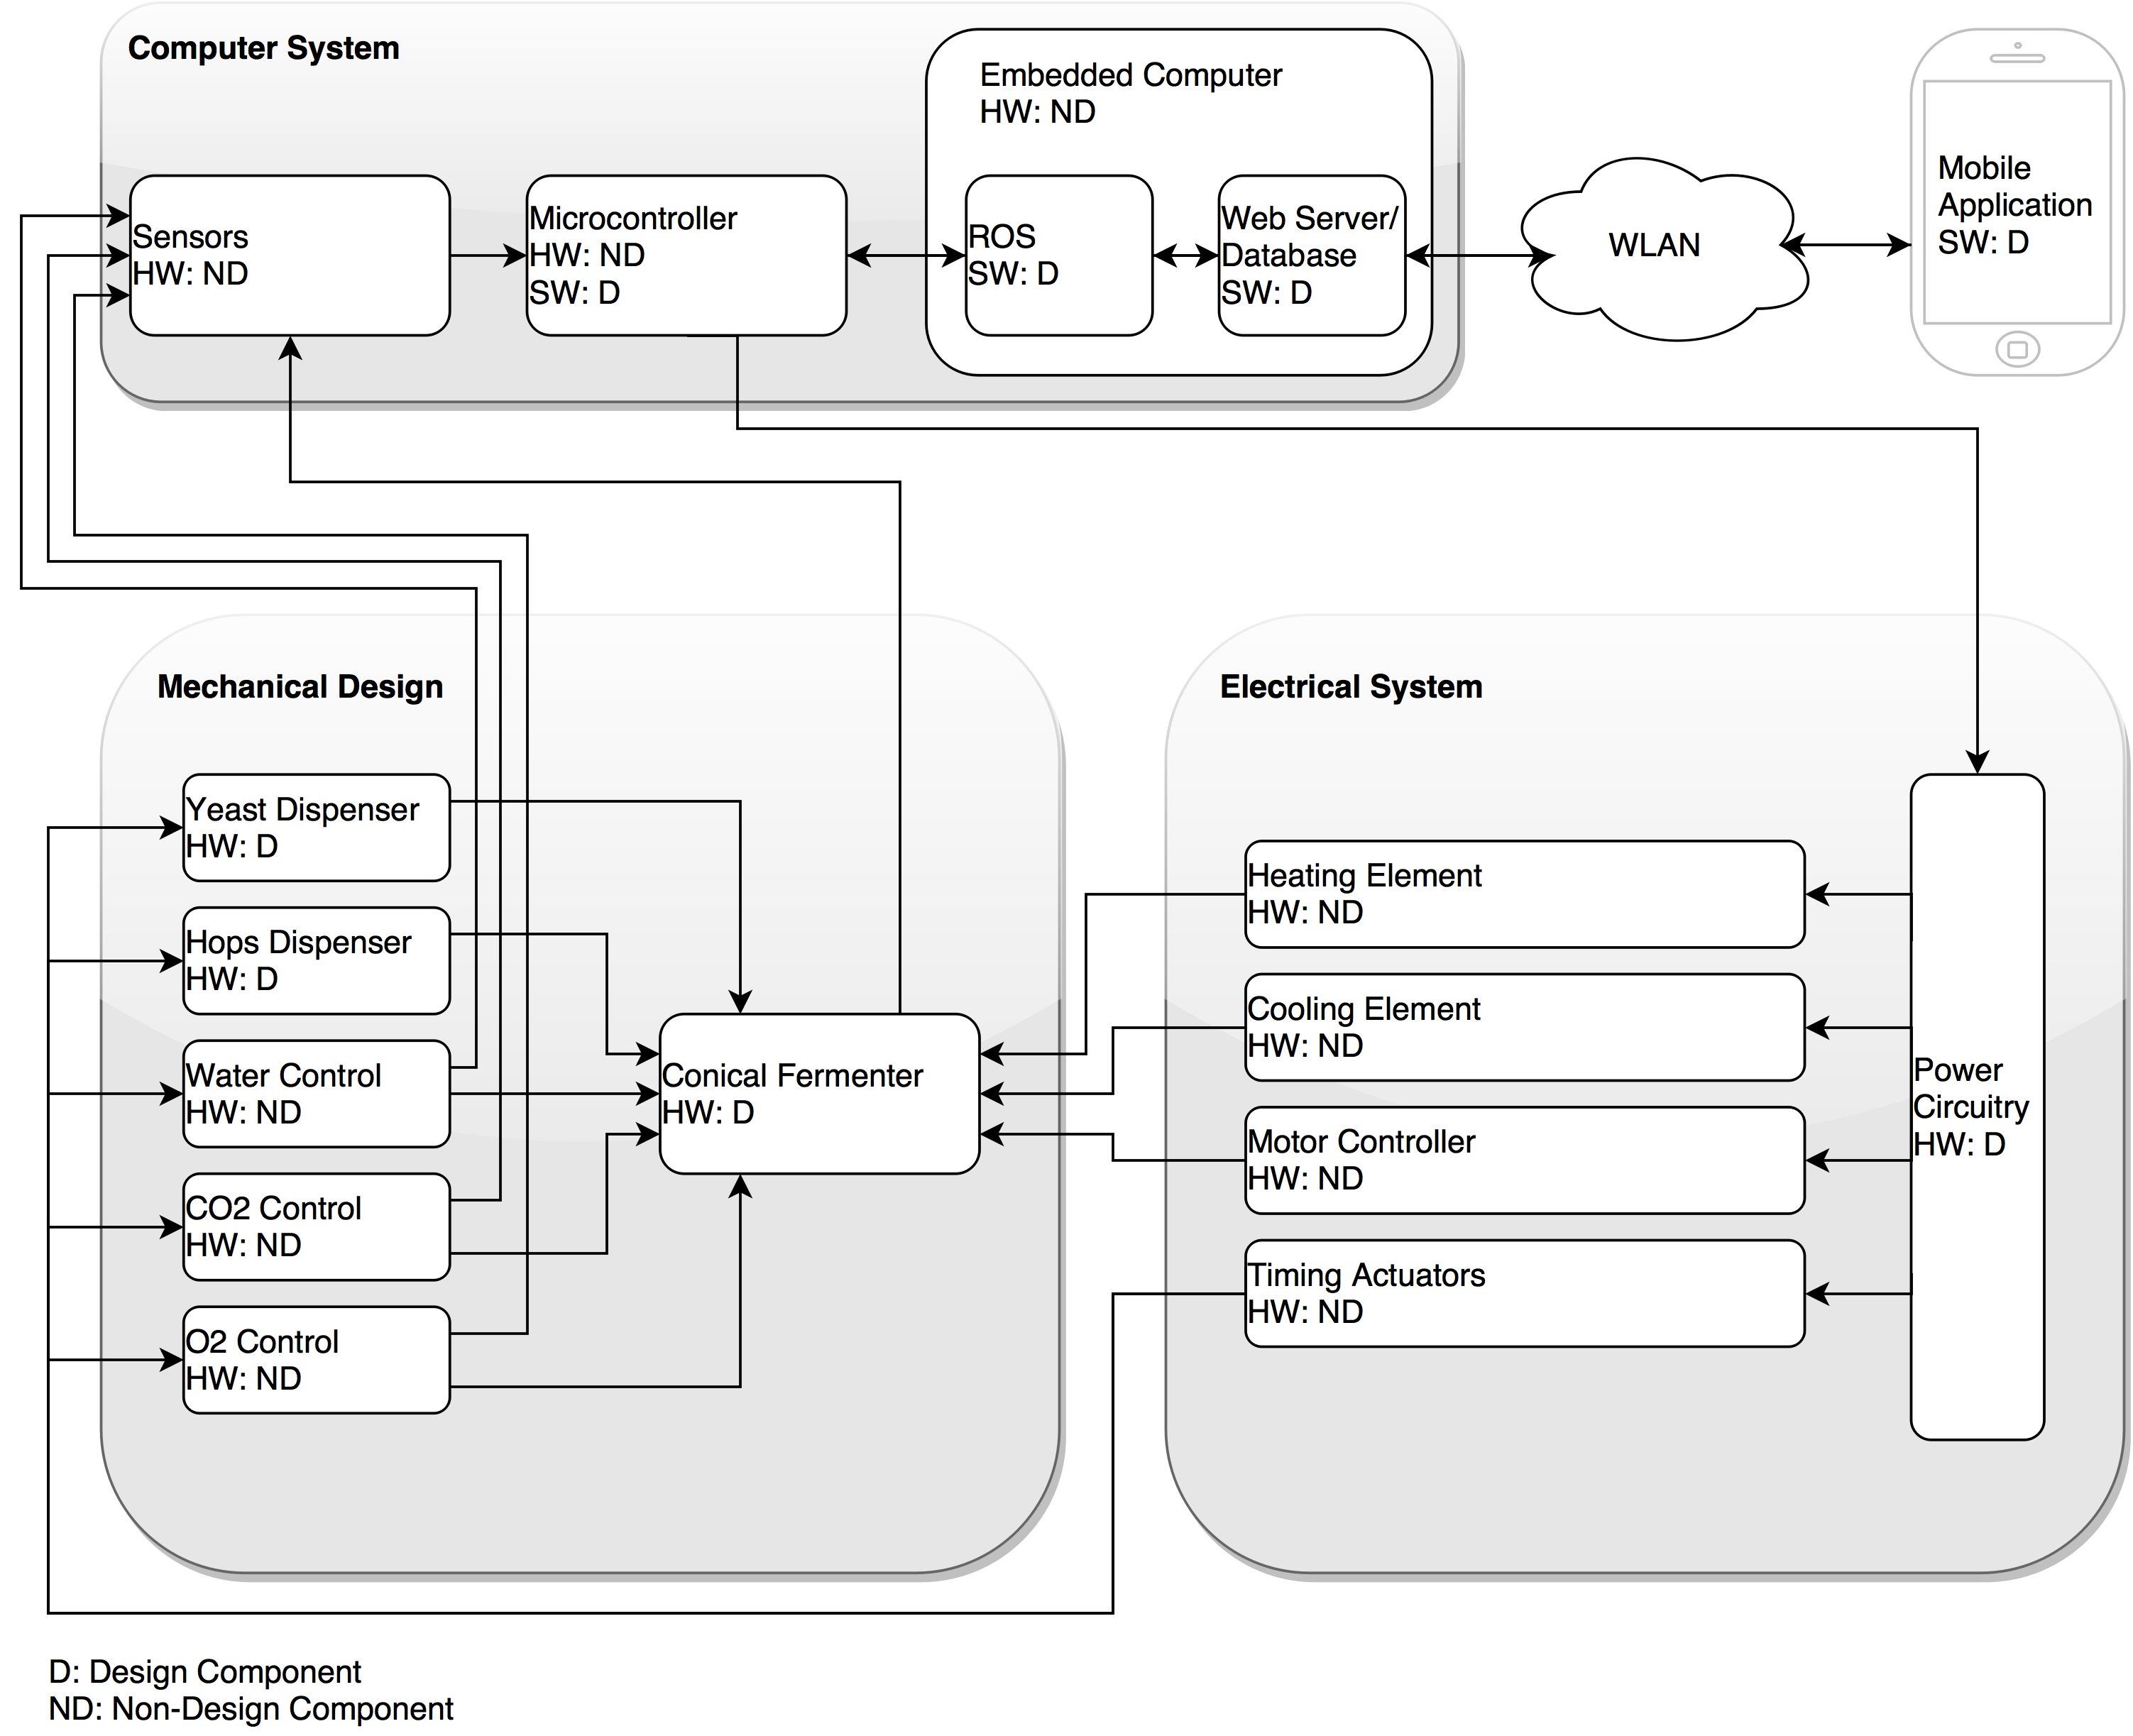
\includegraphics[width=\linewidth]{block-diagram.png}
\caption{Mechanical, electrical, and computer system interactions}
\end{figure}

\end{block}

%----------------------------------------------------------------------------------------
%	REFERENCES
%----------------------------------------------------------------------------------------

\begin{block}{References}

\nocite{*} % Insert publications even if they are not cited in the poster
\small{\bibliographystyle{ieeetr}
\bibliography{poster}\vspace{0.75in}}

\end{block}

%----------------------------------------------------------------------------------------

%----------------------------------------------------------------------------------------
%	ACKNOWLEDGEMENTS
%----------------------------------------------------------------------------------------

\begin{alertblock}{Acknowledgements}

\small{Douglas Harder, Project consultant; \\
Steve Innocente, Technical Assistance; \\
Andrew Svoboda, Brewing Assistance; \\
Baumier, E3 Machine Shop, Fabrication;}

\end{alertblock}

\end{column} % End of the first column

\begin{column}{\sepwid}\end{column} % Empty spacer column

\begin{column}{\twocolwid} % Begin a column which is two columns wide (column 2)

\begin{block}{Mechanical System} 
\end{block}

\begin{columns}[t,totalwidth=\twocolwid] % Split up the two columns wide column

\begin{column}{\onecolwid}\vspace{-.6in} % The first column within column 2 (column 2.1)

%----------------------------------------------------------------------------------------
%	MECHANICAL SYSTEM
%----------------------------------------------------------------------------------------

The American Society of Mechanical Engineers (ASME) outlines a function for determining the wall thickness of a pressure vessel as:

\begin{equation}
t = \frac{P_{work} \times r \times FS}{\sigma_{uts} \times E}
\end{equation}

\noindent Therefore:
\begin{equation}
t = \frac{206.84kpa \times 254mm \times 9}{505MPa \times 0.6}
\end{equation}
\begin{equation}
t = 1.560mm
\end{equation}

The maximum stress experienced by the collar of the outer tank occurs at the inner edge of the collar. 

\scriptsize
\begin{equation}
\sigma = \frac{3w}{mt^{2}(a^{2} - b^{2})}\Big(a^{4}(3m + 1) + b^{4}(m - 1) - 4ma^{2}b^{2} - 4(m + 1)a^{2}b^{2}\ln(\frac{a}{b}) \Big)
\label{eq:stress}
\end{equation}
\normalsize

\noindent Therefore:

\scriptsize
\begin{equation}
t^{2} = \frac{3w}{m\sigma(a^{2} - b^{2})}\Big(a^{4}(3m + 1) + b^{4}(m - 1) - 4ma^{2}b^{2} - 4(m + 1)a^{2}b^{2}\ln(\frac{a}{b}) \Big)
\end{equation}
\normalsize

The resultant thickness is 2.05mm, or 0.08in. Accounting for a safety factor, a sheet thickness of 0.125in. was selected.

%----------------------------------------------------------------------------------------

\end{column} % End of column 2.1

\begin{column}{\onecolwid}\vspace{-.6in} % The second column within column 2 (column 2.2)

%----------------------------------------------------------------------------------------
%	MECHANICAL CONTINUED
%----------------------------------------------------------------------------------------

\begin{figure}
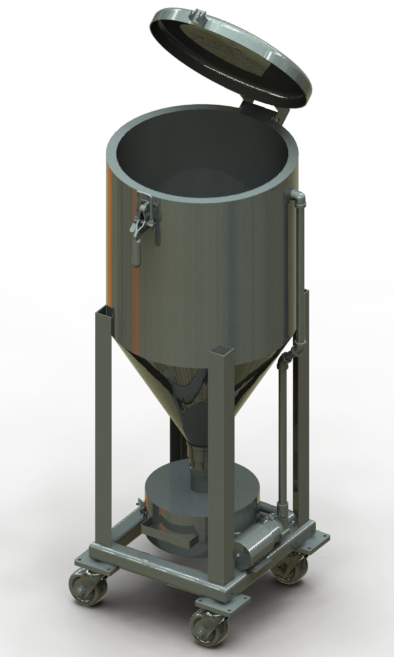
\includegraphics[width=0.56\linewidth]{full-vessel-render.png}
\caption{A mechanical render of the full vessel}
\end{figure}

%----------------------------------------------------------------------------------------

\end{column} % End of column 2.2

\end{columns} % End of the split of column 2 - any content after this will now take up 2 columns width

%----------------------------------------------------------------------------------------
%	BREWING THEORY
%----------------------------------------------------------------------------------------

\begin{alertblock}{Brewing Theory}

The brewing process consists of heating the grains in water to extract the sugars and other flavors (mashing), removing the spent grains but forcing boiling water through them to extract the last sugars (sparging), this sweet water (called wort) is then boiled for sterilization, adding yeast to begin the conversion of the sugars to alcohol (fermentation) and finally treating the product.  During the boiling process, the flower of the hops plant is added for preservation, and to add a bitter flavor.

\end{alertblock} 

%----------------------------------------------------------------------------------------

\begin{block}{Electrical System}
\end{block}

\begin{columns}[t,totalwidth=\twocolwid] % Split up the two columns wide column again

\begin{column}{\onecolwid} % The first column within column 2 (column 2.1)
%----------------------------------------------------------------------------------------
%	ELECTRICAL SYSTEM
%----------------------------------------------------------------------------------------
Since the temperature model of the main volume of water is the same regardless of  temperature change; the cooling system is identical to the heating system with respect to power.

\begin{equation}
Qh = Qs + Ql
\label{eq:heat-system}
\end{equation}

\noindent If differentiated with respect to time, the result is Equation \ref{eq:dt}.

\begin{equation}
P = C \times \frac{dT}{dt} + k(T - T_{a})
\label{eq:dt}
\end{equation}

Taking the Laplace transform of both side, results in Equation \ref{eq:laplace-heat}.

\begin{equation}
P(s) = C \times s \times T(s) + kT(s)
\label{eq:laplace-heat}
\end{equation}

\noindent Resulting in Equation \ref{eq:result-heat}, the transfer function model of the heating of a volume of liquid.

\begin{equation}
\frac{T(s)}{P(s)} = \frac{1}{Cs + k}
\label{eq:result-heat}
\end{equation}

%----------------------------------------------------------------------------------------

\end{column} % End of column 2.1

\begin{column}{\onecolwid} % The second column within column 2 (column 2.2)
%----------------------------------------------------------------------------------------
%	ELECTRICAL CONTINUED
%----------------------------------------------------------------------------------------
\noindent  Finding the value of the parameter C is relatively straightforward, it is equal to the mass of water in the system multiplied by the specific heat capacity of water.

\begin{equation}
C = 50L \times 1\frac{kg}{L} \times 4200\frac{J}{kgK} = 210,000\frac{J}{K}
\label{eq:value-heat}
\end{equation}

\begin{figure}
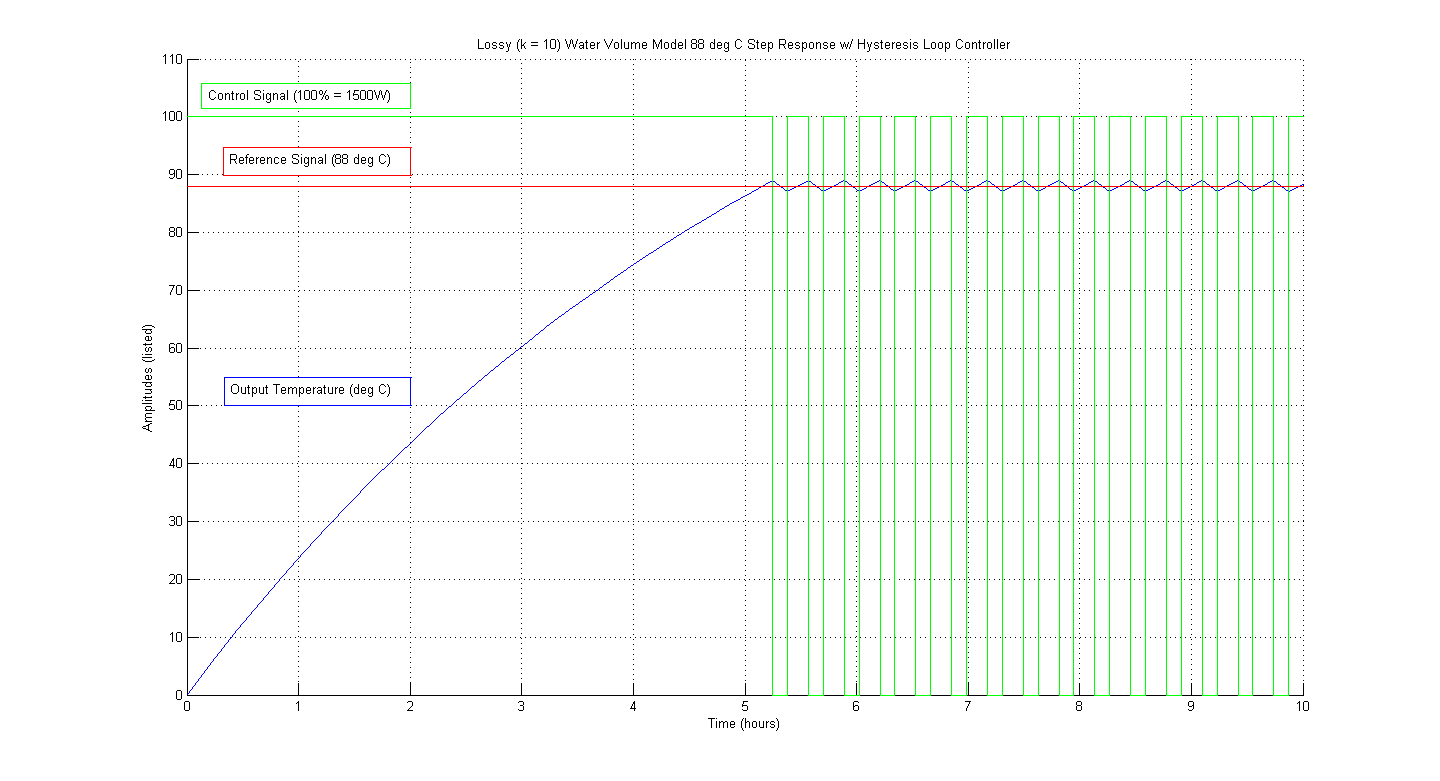
\includegraphics[width=\linewidth]{hysteresis-step-lossy.png}
\caption{Lossy hysteresis loop step response with control signal}
\end{figure}

%----------------------------------------------------------------------------------------

\end{column} % End of column 2.2

\end{columns} % End of the split of column 2

\end{column} % End of the second column

\begin{column}{\sepwid}\end{column} % Empty spacer column

\begin{column}{\onecolwid} % The third column

%----------------------------------------------------------------------------------------
%	NO SPARGE ALGORITHM
%----------------------------------------------------------------------------------------

\begin{block}{No Sparge Algorithm}

The no-sparge technique uses 25\% more grain and allows for the sparging process to be bypassed with no ill effects.  This process greatly reduces the complexity of the process/system and makes the wort more robust and pH stable \cite{sparging}. \\

\noindent The scale up factor is calculated by using Equation \ref{eq:scale-up}.

\begin{equation}
S = \frac{V_{b}}{(V_{b} - kG_{r})}
\label{eq:scale-up}
\end{equation}

\noindent The no-sparge grain-bill is calculated using Equation \ref{eq:grain-bill}.

\begin{equation}
G_{n} = S \times G_{r}
\label{eq:grain-bill}
\end{equation}

\noindent The no-sparge boil gravity is adjusted by using Equation \ref{eq:boil-gravity}.

\begin{equation}
BG = OG \times \frac{V_{r}}{V_{b}}
\label{eq:boil-gravity}
\end{equation}

\noindent The total no-sparge water volume in quarts is determined by Equation \ref{eq:water-volume}.

\begin{equation}
W_{n} = 4(V_{b} + kG_{n})
\label{eq:water-volume}
\end{equation}

\noindent By using Equation \ref{eq:mash-ratio} the no-sparge mash ratio is calculated.

\begin{equation}
R_{n} = \frac{W_{n}}{G_{n}}
\label{eq:mash-ratio}
\end{equation}

\noindent The volume of water used for the mash-out in quarts is determined by Equation \ref{eq:water-mashout}.

\begin{equation}
W_{mo} = G_{n}(R_{n} - R_{r})
\label{eq:water-mashout}
\end{equation}

\noindent Finally, the total no-sparge mash volume in quarts is calculated using Equation \ref{eq:mash-volume}.

\begin{equation}
V_{t} = G_{n}(1.3125 + (R_{n} - 1)
\label{eq:mash-volume}
\end{equation}

\end{block}

%----------------------------------------------------------------------------------------
%	ADDITIONAL INFORMATION
%----------------------------------------------------------------------------------------

\begin{alertblock}{Additional Information}

\begin{figure}
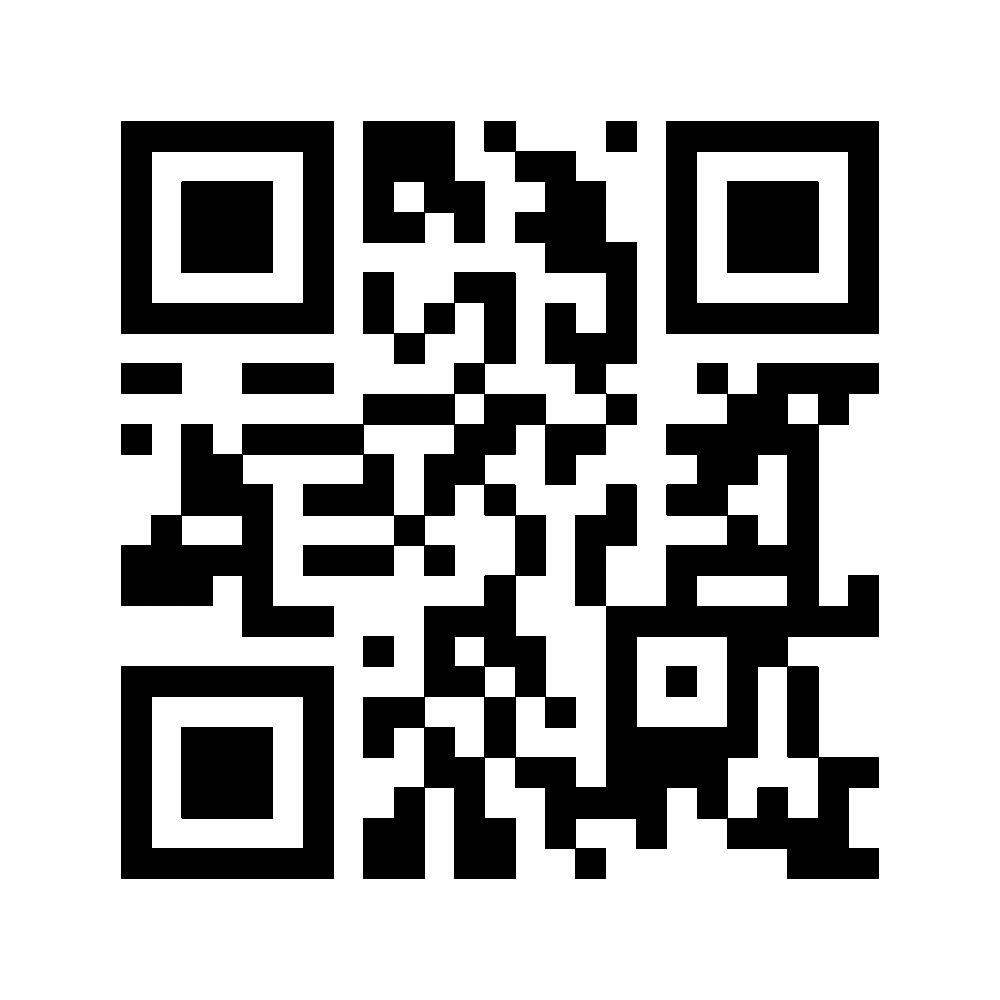
\includegraphics[width=0.4\linewidth]{qr-biy.png}
\caption{\href{https://github.com/BrewItYourself}{github.com/BrewItYourself}}
\end{figure}

\end{alertblock}

\begin{flushright}
Group 2016.019 - Brew It Yourself
\end{flushright}

%----------------------------------------------------------------------------------------

\end{column} % End of the third column

\begin{column}{\sepwid}\end{column} % Empty spacer column

\end{columns} % End of all the columns in the poster

\end{frame} % End of the enclosing frame

\end{document}
